\chapter{Разработка прототипа}
В данном разделе описываются значимые детали реализации прототипа метода редукции програм на языке Kotlin. Основное применение прототипа --- редукция ошибок компилятора языка Kotlin. Источником информации в этом разделе является исходный код прототипа, частично представленный в приложении.
\section{Архитекура прототипа}
Разрабатываемый прототип основывается на предложенной технологии. Прототип разрабатывался на языке программирования Kotlin. Общая структура пакетов представлена на рисунке~\ref{packages}. Как видно из диаграммы, прототип состоит из следующих основных частей:
\begin{itemize}
	\item \texttt{manager} --- отвечает за запуск трансформаций и обработку результатов;
	\item \texttt{parser} --- отвечает за построение синтаксического дерева;
	\item \texttt{passes} --- содержит реализацию всех трансформаций;
	\item \texttt{util} --- содержит вспомогательные компоненты.
\end{itemize}
Далее реализация прототипа рассмотрена более детально.

\begin{figure}
\center{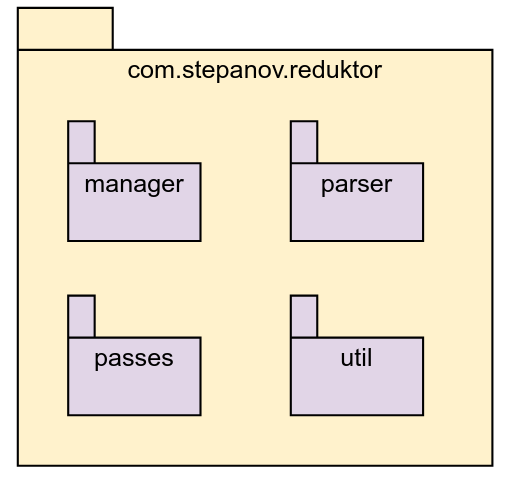
\includegraphics[width=0.5\linewidth]{fig/packages}}
\caption{\label{packages}Общая структура пакетов прототипа}
\end{figure}

\section{Реализация инструмента для построения PSI}
В пакете \texttt{parser} содержится код, предназначенный для построения СД из исходного кода языка программирования Kotlin. Путь к исходному коду задается через программный аргумент \texttt{--path}. Построение производится путем использования инструментария компилятора Kotlin. Для каждого файла с исходным кодом строится свое СД. Стоит отметить, что для прохода по СД и его редактирования также используется функциональность компилятора Kotlin.

Как было написано ранее, язык программирования Kotlin полностью совместим с языком Java. В качестве дополнительной функциональности было реализовано получение СД для кода на языке программирования Java, так как большое количество программ являются мультиплатформенными, то есть имеющими код как на языке Kotlin, так и на языке Java. Поэтому для редукции таких проектов будет необходимо обрабатывать и код на языке Java. 

\section{Реализация редуцирующих трансформаций}
В пакете \texttt{passes} содержатся все редуцирующие трансформации. Каждая трансформация принимает на вход какое-либо представление кода и всю необходимую информацию и обрабатывает его. То есть на выходе они дают программу, которая приводит к той же ошибке, что и поданная на вход, но только имеющую меньший размер. Все реализованные алгоритмы соотвествуют описанным в предыдущей главе. Ниже приведены особенности реализации некоторых из них.

Класс \texttt{ParallelHierarchialDeltaDebugging} реализует параллельный дельта дебаггинг СД путем запуска в отдельных потоках обработки различных уровней дерева. Эксперименты показали, что данная доработка не ускоряет работу метода из-за того что, при удалении более высокоуровнего объекта происходит исключение из обработки большого количества низкоуровневых. И почти всегда количество обрабатываемых дополнительно низкоуровневых элементов настолько велико, что перекрывает преимущества параллельной обработки. Путь решения данной проблемы --- при удалении какого-либо элемента сообщать всем нижним уровням и исключать из рассмотрения всех детей удаленного элемента. Но при этом редукцию на этих уровнях нужно будет запускать заново. Из-за этого распараллеливание дельта дебаггинга на уровнях дерева разбора можно считать нецелесообразным. 

Класс \texttt{PeepholePasses} реализует все алгоритмы редукции текстового представления программы. Шаблоны, описанные в предыдущей главе, задаются при помощи регулярных выражений. Единственная проблема, возникшая в процессе разработки --- скобки могут быть несбалансированными, например, находиться в строковых константах. Эти случаи были отдельно обработаны.

Класс \texttt{PreliminarySimplification} реализует алгоритм предварительного упрощения файлов. Очевидно, что для ускорения работы данный алгоритм может быть распареллелен --- каждый файл может обрабатываться отдельно. Экспериментальным путем был выделен следующий набор трансформаций для предварительного упрощения файлов:
\begin{itemize}
	\item упрощение функций и свойств;
	\item трансформации над текстовым представлением программы;
	\item удаление пустых управляющих конструкций;
	\item удаление неиспользуемых импортирований.
\end{itemize}


\subsection{Пакет com.stepanov.reduktor.passes.slicer}
Данный пакет содержит в себе классы, реализующие алгоритмы программных срезов, описанные в предыдущем разделе. Пакет содержит класс \texttt{Slicer}, который принимает на вход номер строки с ошибкой и запускает выбранный вид слайсинга. Для получения переменных по номеру строки была написана функция \texttt{getline}, которая обходит дерево разбора в глубину, считая количество переводов строки, в нужный момент останавливается и извлекает имена всех использующихся в этой строке переменных. 

Как было описано ранее, внутрипроцедурный слайсер обходит тело функции снизу вверх и удаляет все то, что не относится к критерию среза. Данный проход имеет несколько особенностей реализации:
\begin{itemize}
	\item если в критерии среза содержится номер строки, указывающей на вызов функции, то в качестве переменных в критерии среза используются аргументы, переданные в функцию;
	\item если известна только функция, в которой содержится ошибка, то, ввиду скорости работы слайсера, поочередно производится срез относительно каждой строки этой функции;
	\item для безопасности слайсинга определен четкий набор обрабатываемых видов выражений(унарное, бинарное, вызов функции и т.д.), также отдельно обрабатываются блоки.
\end{itemize}

Слайсер на уровне функций работает по алгоритму, описанному в главе 3 --- строит дерево использований функций, где корнем является функция с ошибкой и удаляет все функции, которые не попали в это дерево. Для реализации построения дерева необходимо соотнести вызов функции с её сигнатурой. Так как при редукции компиляторных ошибок анализ кода часто не может быть проведен, не имеется никакой информации о типах аргументов в вызове функции, если они не указаны явно. Для решения этой проблемы была написана функция \texttt{getSignature}, которая считает количество аргументов, и дальнейший поиск производится по имени функции и количеству ее аргументов. Очевидно, что иногда такой подход будет строить неверные деревья, поэтому перед удалением каждой функции производится проверка корректности удаления. Также стоит отметить, что дерево строится с фильтрацией рекурсивных вызовов.

\section{Реализация менеджера проходов}
В пакете \texttt{reducer} содержится компонент \texttt{TransformationManager}, реализующий управление всеми трансформациями. Данный компонент осуществляет запуск наборов трансформаций для проектов (\texttt{doProjectTransformations}) и отдельных файлов (\texttt{doTransformations}). Трансформации запускаются в цикле до тех пор, пока файл с ошибкой не перестанет изменяться. Также данный компонент отвечает за постобработку результатов --- форматирование и сохранение.  Для форматирования результирующего кода был апробирован проект ktlint\footnote{https://github.com/shyiko/ktlint}, но его применение не дало ожидаемых результатов. После этого была попытка интегрировать модуль редактирования стиля кода из среды разработки IDEA~\footnote{https://www.jetbrains.com/idea/} и компилятора Kotlin, но ввиду сложности внутренних связей данного модуля его интеграция не является целесообразной. Поэтому была реализована трансформация, удаляющая лишние переводы строк, а для полного форматирования можно использовать функциональность среды разработки IDEA. 

\section{Реализация вспомогательных компонентов}
Пакет \texttt{util} содержит вспомогательные компоненты, решающие следующие задачи:
\begin{itemize}
	\item запуск программы и проверка воспроизведения ошибки \texttt{CompilatorCrushTestChecker};
	\item дерево для хранения объектов любого типа --- \texttt{DependencyTree};
	\item хранение аргументов, с которым запускается компилятор --- \texttt{CompilerArgs};
	\item разбор сообщения об ошибке и ее хранение --- \texttt{Error};
	\item распараллеливание задач любых видов на уровне файлов --- \texttt{ParralelFileProcessingUtil};
	\item удаление файлов исходного кода из архива с зависимостями --- \texttt{RemoveSourcesFromJar};
	\item дополнительные инструменты для редактирования СД --- \texttt{Extensions}.
\end{itemize}
Ниже приведено описание наиболее интересных компонентов.

\subsection{Компонент \texttt{CompilatorCrushTestChecker}}
Так как основным применением разработанного протоипа является редукция программ, приводящих к ошибкам компилятора, был разработан отдельный компонент для запуска программ и проверки воспроизведения ошибок. Для запуска программы используется компонент \texttt{K2JVMCompiler} из компилятора языка Kotlin. С помощью компонента \texttt{CompilerArgs} задаются все необходимые аргументы и производится запуск компилятора с использованием библиотеки \texttt{java.util.concurrent}. Результат запуска сохраняется в специальную структуру \texttt{MessageCollector}, содержащую всю необходимую инфомрацию об ошибке. Далее происходит разбор ошибки, и сравнение ее с исходной. В том случае, если сообщение об ошибке не подходит ни под один заданный шаблон, сраниваются текстовые представления ошибок алгоритмом, описанным в главе 3. Для сравнения используется библиотека \texttt{DiffMatchPatch}, после чего считается коэффициент схожести файлов и сравнивается с заданным коэффициентом, который подбирался экспериментально. 

В описываемом компоненте содержатся две доработки для многократного повышения скорости работы прототипа. Первая --- сохранение уже проверенных конфигураций. Для этого используется хэш-таблица, содержащая хэш-код проверенных конфигураций и результат их проверки. Второй --- проверка синтаксической корректности запускаемого теста, и, если тест некорректен, он пропускается. Для данной проверки используется инструментарий компилятора Kotlin: если текст программы некорректен, синтаксическое дерево для нее содержит специальный вид узлов, сингализирующих об этом. 

\subsection{Компонент \texttt{ParallelFileProcessingUtil}}
Данный компонент реализует параллельный запуск задач на выполнение. Для распараллеливания используется стандартный пакет \texttt{java.util.concurrent}, содержащий все необходимые для этого инструменты. Количество потоков равно количеству процессоров компьютера. Для каждого потока создается копия проекта, после обработки новый файл сохраняется в старый проект. В проекте используются два вида параллельных задач: быстрое упрощение и набор трансформаций, описанных в компоненте \texttt{PreliminarySimplification}. Быстрое упрощение состоит в попытке замены тел всех функций на вызов специальной функции TODO(). В случае, если все функции не влияют на воспроизведение ошибки, производится удаление их тел, что значительно уменьшает размер обрабатываемого кода. 

\subsection{Компонент \texttt{RemoveSourcesFromJar}}
Для запуска программы для проверки воспроизведения ошибки компоненту~\texttt{K2JVMCompiler} необходимо передать архив со всеми зависимостями целевого проекта. Данный архив практически всегда содержит и скомпилированный исходный код программы. Это приводит к тому, что при удалении какого-либо компонента программы из исходного кода, он все равно <<подхватывается>> из указанного архива. Описанная ситуация приводит к невозможности воспроизведения ошибки результирующим тестовым примером. Данный компонент занимается удалением всех скомпилированных элементов исходного кода из архива с зависимостями.

\section{Резюме}
В данном разделе были описаны компоненты, реализующие предложенный подход редукции программ на языке Kotlin. Исходный код для некоторых описанных компонентов приведен в приложении Б.